%!Mode:: "TeX:UTF-8"
\documentclass{beamer}
\usepackage{xeCJK}
\usepackage{xcolor}
\usepackage{listings}
\usepackage{soul}
\usepackage{ulem}

\setCJKmainfont{AR PL SungtiL GB}

\definecolor{dkgreen}{rgb}{0,0.6,0}
\definecolor{gray}{rgb}{0.5,0.5,0.5}
\definecolor{mauve}{rgb}{0.58,0,0.82}

\lstset{
    language=sh,
    %basicstyle=\footnotesize\ttfamily,
    basicstyle=\scriptsize\ttfamily,
    frameround=tttt,
    frame=single,
    keywordstyle=\color{blue},
    commentstyle=\color{dkgreen},
    stringstyle=\color{mauve},
    numbers=left,
    numberstyle=\tiny\color{gray},
    numbersep=5pt,
    escapeinside={(*@}{@*)},
    %otherkeywords={$, \{, \}, \[, \]},
}

%\setbeamertemplate{footline}[frame number]
\setbeamertemplate{navigation symbols}{}
\usetheme{Madrid}
\begin{document}

\title{Git + Trac + Dyb2Sim}
\author{
    \texorpdfstring{林韬
                    \newline
                    \href{mailto:lintao@ihep.ac.cn}
                    {\footnotesize\ttfamily{lintao@ihep.ac.cn}}}
                    {Lin Tao}
}

\institute{IHEP}

\maketitle

\begin{frame}
    \frametitle{OUTLINE}
    \tableofcontents
\end{frame}

\section{Quick Start}
    %!Mode:: "TeX:UTF-8"
%\begin{frame}
%    \frametitle{OUTLINE}
%    \begin{itemize}    
%        \item
%    \end{itemize}
%\end{frame}

\begin{frame}
    \begin{center}
        \LARGE \tt{Quick Start}
    \end{center}
\end{frame}

\newsavebox{\QuickStartEnvSetup}
\begin{lrbox}{\QuickStartEnvSetup}
\begin{lstlisting}
Login lxslc5.ihep.ac.cn
$ mkdir ~/tutProject
$ cd ~/tutProject
create bashrc which contains Line 6 to 8
$ cat bashrc 
source /panfs/panfs.ihep.ac.cn/home/dyb/dybsw/dyb2/external/local/bashrc
export G4WORKDIR=~/geant4
export PATH=${G4WORKDIR}/bin/Linux-g++:$PATH
$ source bashrc
\end{lstlisting}
\end{lrbox}

\newsavebox{\QuickStartGitClone}
\begin{lrbox}{\QuickStartGitClone}
\begin{lstlisting}
$ git clone (*@{\color{red}-o ltrepo}@*) git@dyb2app1.ihep.ac.cn:users/lintao/Dyb2Sim
\end{lstlisting}
\end{lrbox}

\begin{frame}
    \frametitle{环境设置 \&\& clone代码}
    \begin{block}{环境设置}
        \par\usebox{\QuickStartEnvSetup}
    \end{block}
    \begin{block}{导出代码}
        \par\usebox{\QuickStartGitClone}
    \end{block}
    \begin{alertblock}{提示}
        \begin{itemize}    
            \item {\tt -o ltrepo}是给远程仓库设定别名,因此,名字可任意
        \end{itemize}
    \end{alertblock}
\end{frame}

\newsavebox{\QuickStartDybCompile}
\begin{lrbox}{\QuickStartDybCompile}
\begin{lstlisting}
$ cd Dyb2Sim/DetSim/DetSim0
$ make
\end{lstlisting}
\end{lrbox}

\newsavebox{\QuickStartDybRun}
\begin{lrbox}{\QuickStartDybRun}
\begin{lstlisting}
$ dyb2main run.mac
\end{lstlisting}
\end{lrbox}

\newsavebox{\QuickStartDybRunMore}
\begin{lrbox}{\QuickStartDybRunMore}
\begin{lstlisting}
$ cd mac/
$ ls
\end{lstlisting}
\end{lrbox}

\begin{frame}
    \frametitle{编译 \&\& 运行}
    \begin{block}{编译}
        \par\usebox{\QuickStartDybCompile}
    \end{block}
    \begin{block}{运行}
        \par\usebox{\QuickStartDybRun}
    \end{block}
    \begin{block}{运行更多的mac文件}
        \par\usebox{\QuickStartDybRunMore}
    \end{block}
\end{frame}

\newsavebox{\QuickStartDybGeneratorCompile}
\begin{lrbox}{\QuickStartDybGeneratorCompile}
\begin{lstlisting}
$ pwd
(*@{\color{red}/afs/ihep.ac.cn/users/l/lint/}@*)tutProject/Dyb2Sim/DetSim/DetSim0/mac
$ cd ../../../Generator/InverseBeta/
$ make
$ ls
GNUmakefile  (*@{\color{green}IBD}@*)  include  src
\end{lstlisting}
\end{lrbox}

\newsavebox{\QuickStartDybGeneratorRun}
\begin{lrbox}{\QuickStartDybGeneratorRun}
\begin{lstlisting}
$ ./IBD --help
查看帮助
$ ./IBD -o (*@{\color{red}ibd.asc}@*) -n 1000
$ cp ibd.asc ../../DetSim/DetSim0/mac/
$ cd ../../DetSim/DetSim0/mac/
$ head run_hepevt_ibd.mac -n 3
/dyb2/gen/source/reset

/dyb2/gen/source/HepEvt/append (*@{\color{red}ibd.asc}@*)
$ dyb2main run_hepevt_ibd.mac 
\end{lstlisting}
\end{lrbox}

\begin{frame}
    \frametitle{编译 \&\& 运行 产生子}
    \begin{block}{编译}
        \par\usebox{\QuickStartDybGeneratorCompile}
    \end{block}
    \begin{block}{运行}
        \par\usebox{\QuickStartDybGeneratorRun}
    \end{block}
\end{frame}

\newsavebox{\QuickStartDybDevRemote}
\begin{lrbox}{\QuickStartDybDevRemote}
\begin{lstlisting}
$ git remote show 
(*@{\color{red}ltrepo}@*)
$ git remote add (*@{\color{red}ownrepo}@*) git@dyb2app1.ihep.ac.cn:users/(*@{\color{red}lintao}@*)/(*@{\color{red}tutProject}@*)
$ git remote show 
(*@{\color{red}ltrepo}@*)
(*@{\color{red}ownrepo}@*)
\end{lstlisting}
\end{lrbox}

\begin{frame}
    \frametitle{开发}
    \begin{itemize}    
        \item 根据不同的方案,建立不同的\tt{DetSim{\color{red}X}}
        \item 暂时将\tt{DetSim0}作为开发的模板
        \item 开发一个新任务时,尽量创建新的分支
        \item 把自己本地代码,push到git服务器
    \end{itemize}
\end{frame}

\begin{frame}
    \frametitle{设置远程仓库}
    \begin{itemize}    
        \item 此处,讲解如何添加远程仓库
        \item 目前的策略:每个人可以往自己的目录下{\Large 写入}或{\Large 添加}项目
        \item 其他开发者可以{\Large 读取}你的项目
    \end{itemize}
    \begin{block}{示例}
        \par\usebox{\QuickStartDybDevRemote}
    \end{block}
    \begin{alertblock}{提示}
        \begin{itemize}    
            \item {\tt ownrepo}是给远程仓库设定别名
            \item {\tt lintao}是申请时的账户
            \item {\tt tutProject}是项目的名称
        \end{itemize}
    \end{alertblock}
\end{frame}

\newsavebox{\QuickStartDybDevBranch}
\begin{lrbox}{\QuickStartDybDevBranch}
\begin{lstlisting}
$ git branch 
* master
$ git checkout -b (*@{\color{red}lintao-dev}@*)
Switched to a new branch '(*@{\color{red}lintao-dev}@*)'
$ git branch 
* (*@{\color{red}lintao-dev}@*)
  master
\end{lstlisting}
\end{lrbox}

\begin{frame}
    \frametitle{创建新的分支}
    \begin{itemize}    
        \item 分支的创建是为了不影响其他人的开发
        \item 保留master分支,便于合并
        \item 创建自己的dev分支,此分支应该push到服务器
        \item 创建其他分支时,最好从自己的dev分支开始
    \end{itemize}
    \begin{block}{示例}
        \par\usebox{\QuickStartDybDevBranch}
    \end{block}
    \begin{alertblock}{提示}
        \begin{itemize}    
            \item {\tt git checkout -b}表示导出一个新的branch
            \item 如果分支已经存在,只要{\tt git checkout}
        \end{itemize}
    \end{alertblock}
\end{frame}

\newsavebox{\QuickStartDybDevBranchPush}
\begin{lrbox}{\QuickStartDybDevBranchPush}
\begin{lstlisting}
$ git push (*@{\color{red}ownrepo}@*) (*@{\color{red}lintao-dev}@*)
... skip ...
To git@dyb2app1.ihep.ac.cn:users/lintao/tutProject
 * [new branch]      lintao-dev -> lintao-dev
\end{lstlisting}
\end{lrbox}

\newsavebox{\QuickStartDybDevBranchFetch}
\begin{lrbox}{\QuickStartDybDevBranchFetch}
\begin{lstlisting}
$ git fetch (*@{\color{red}ltrepo}@*)
\end{lstlisting}
\end{lrbox}

\begin{frame}
    \frametitle{更多关于分支的常用操作}
    \begin{block}{push分支至服务器}
        \par\usebox{\QuickStartDybDevBranchPush}
    \end{block}
    \begin{block}{同步远程服务器仓库}
        \par\usebox{\QuickStartDybDevBranchFetch}
    \end{block}
    \begin{alertblock}{提示}
        \begin{itemize}    
            \item {\tt git push}表示把当前的分支{\color{red}lintao-dev}推送到仓库{\color{red}ownrepo}
            \item 对于不想分享的分支,就不要推送了
            \item {\tt git fetch},是为了更新远程仓库的本地备份,并与{\color{red}ltrepo}同步
            \item 在多开发者的情况下,添加多个remote,可以方便同步
        \end{itemize}
    \end{alertblock}
\end{frame}

\newsavebox{\QuickStartDybDevCommit}
\begin{lrbox}{\QuickStartDybDevCommit}
\begin{lstlisting}
$ git commit -am '(*@{\color{red}Comment}@*)' 
\end{lstlisting}
\end{lrbox}

\newsavebox{\QuickStartDybDevStatus}
\begin{lrbox}{\QuickStartDybDevStatus}
\begin{lstlisting}
$ git status
$ git diff
$ gitk
\end{lstlisting}
\end{lrbox}

\begin{frame}
    \frametitle{本地工作目录常用命令}
    \begin{block}{记录每次更新到本地仓库}
        \par\usebox{\QuickStartDybDevCommit}
    \end{block}
    \begin{block}{查看工作目录的改动}
        \par\usebox{\QuickStartDybDevStatus}
    \end{block}
    \begin{alertblock}{提示}
        \begin{itemize}    
            \item 在开发过程中,本页是最常用的命令
            \item 最好让自己的代码处于跟踪状态
            \item 另外,如果有图形X,可以使用\tt{gitk}查看历史
        \end{itemize}
    \end{alertblock}
\end{frame}

\newsavebox{\QuickStartDybDevPull}
\begin{lrbox}{\QuickStartDybDevPull}
\begin{lstlisting}
$ git pull (*@{\color{red}ownrepo}@*) (*@{\color{red}lintao-dev}@*)
\end{lstlisting}
\end{lrbox}

\begin{frame}
    \frametitle{同步仓库}
    \begin{block}{使用\tt{git pull}进行同步合并}
        \par\usebox{\QuickStartDybDevPull}
    \end{block}
    \begin{alertblock}{提示}
        \begin{itemize}    
            \item \tt{git pull}可认为是\tt{git fetch}后再\tt{git merge}
            \item 即把远程仓库的分支合并到了本地仓库的相应分支中
            \item 对于同步你个人的仓库,可以使用\tt{git pull}简化操作
                \begin{itemize}
                    \item 多份指向同一远程仓库的工作目录
                \end{itemize}
        \end{itemize}
    \end{alertblock}
\end{frame}

\newsavebox{\QuickStartDybDevMerge}
\begin{lrbox}{\QuickStartDybDevMerge}
\begin{lstlisting}
$ git branch 
* lintao-dev
  master
$ git checkout -b lintao-tut-1
$ git checkout -b lintao-tut-2
$ git branch 
  lintao-dev
  lintao-tut-1
* lintao-tut-2
  master
\end{lstlisting}
\end{lrbox}

\begin{frame}
    \frametitle{分支的合并}
    \begin{block}{使用\tt{git checkout -b}创建分支}
        \par\usebox{\QuickStartDybDevMerge}
    \end{block}
    \begin{alertblock}{提示}
        \begin{itemize}    
            \item \tt{git branch}可以查看分支的状况
        \end{itemize}
    \end{alertblock}
\end{frame}

\newsavebox{\QuickStartDybDevMergeCont}
\begin{lrbox}{\QuickStartDybDevMergeCont}
\begin{lstlisting}
$ touch TUT_TMP
$ ls
DetSim  Generator  README  (*@{\color{red}TUT\_TMP}@*)
$ git add TUT_TMP
$ git commit -am 'Add TUT_TMP in lintao-tut-2.'
$ git checkout lintao-tut-1 
Switched to branch 'lintao-tut-1'
$ ls
DetSim  Generator  README
$ git merge lintao-tut-2 
$ ls
DetSim  Generator  README  (*@{\color{red}TUT\_TMP}@*)
\end{lstlisting}
\end{lrbox}

\begin{frame}
    \frametitle{分支的合并}
    \begin{block}{使用\tt{git merge}进行合并}
        \par\usebox{\QuickStartDybDevMergeCont}
    \end{block}
    \begin{alertblock}{提示}
        \begin{itemize}    
            \item 不同的分支互不影响
            \item \tt{git merge}可在不同的分支间进行合并
        \end{itemize}
    \end{alertblock}
\end{frame}

\newsavebox{\QuickStartSummary}
\begin{lrbox}{\QuickStartSummary}
\begin{lstlisting}
$ dyb2main run.mac
$ ./IBD -o (*@{\color{red}ibd.asc}@*) -n 1000
$ git clone (*@{\color{red}-o ltrepo}@*) git@dyb2app1.ihep.ac.cn:users/lintao/Dyb2Sim
$ git remote show 
$ git remote add (*@{\color{red}ownrepo}@*) git@dyb2app1.ihep.ac.cn:users/(*@{\color{red}lintao}@*)/(*@{\color{red}tutProject}@*)
$ git checkout -b (*@{\color{red}lintao-dev}@*)
$ git push (*@{\color{red}ownrepo}@*) (*@{\color{red}lintao-dev}@*)
$ git pull (*@{\color{red}ownrepo}@*) (*@{\color{red}lintao-dev}@*)
$ git commit -am '(*@{\color{red}Comment}@*)' 
$ git status
$ git diff
$ git merge lintao-tut-2 
$ gitk
\end{lstlisting}
\end{lrbox}

\begin{frame}
    \frametitle{小结}
        \begin{itemize}
            \item 本节主要涉及了一些常用的操作
            \item 涉及最多的便是\tt{git}这个工具
            \item 希望能够帮助大家把程序运行起来
            \item 并了解开发时如何使用这个工具
        \end{itemize}
        \begin{block}{常用命令回顾}
            \par\usebox{\QuickStartSummary}
        \end{block}
\end{frame}

\section{Dyb2Sim}
    %!Mode:: "TeX:UTF-8"
\begin{frame}
    \begin{center}
        \LARGE \tt{基于Sniper的Dyb2Sim}
    \end{center}
\end{frame}

%\begin{frame}
%    \frametitle{OUTLINE}
%    \begin{itemize}    
%        \item
%    \end{itemize}
%\end{frame}

\begin{frame}
    \frametitle{简介}
    \begin{itemize}    
        \item Sniper是新的软件框架,追求简洁,适合非对撞实验。
        \item 主要提供了算法,服务和工具。
        \item 我们的工作是将探测器模拟程序整合到框架中。
        \item 参考邓子艳老师的工作,对Geant4中{\tt RunManager}进行了改造。
              使其更适合于Sniper这个框架的工作行为。
        \item 但和BOSS中有所不同。我将不同的探测器模拟程序抽象为一个算法,
              使用抽象工厂实现与不同模拟程序的连接。
        \item 即原有的geant4程序无需做任何修改,只需要提供一个抽象工厂,
              这样基于Sniper的DetSim会根据此工厂自动构建探测器。
    \end{itemize}
\end{frame}

\newsavebox{\NoviceJobOptions}
\begin{lrbox}{\NoviceJobOptions}
\begin{lstlisting}
#include "$DETSIMROOT/share/jobOptions.txt"
Sniper.Dlls += {"Novice01"};
SvcMgr.Contents += {"ExN01Factory"};

Sniper.Cycler = "NormCycler";
Sniper.InputSvc = "NONE";

DetSim.DetFactory = "ExN01Factory";
DetSim.RunMac = "run.mac";

Sniper.EvtMax   = 2;
Sniper.LogLevel = 3; // INFO
\end{lstlisting}
\end{lrbox}

\begin{frame}
    \frametitle{Geant4 Novice01的整合:job option文件}
    \par\usebox{\NoviceJobOptions}
\end{frame}

\newsavebox{\NoviceHeader}
\begin{lrbox}{\NoviceHeader}
\begin{lstlisting}
class ExN01Factory:  virtual public SvcBase , 
                     virtual public IDetSimFactory {
public:
    ExN01Factory(const std::string& name);
    virtual ~ExN01Factory();

    virtual G4VUserDetectorConstruction* createDetectorConstruction();
    virtual G4VUserPhysicsList* createPhysicsList();
    virtual G4VUserPrimaryGeneratorAction* createPrimaryGenerator();

    virtual bool initialize();
    virtual bool finalize();
};
\end{lstlisting}
\end{lrbox}

\begin{frame}
    \frametitle{Novice 01 需要提供的抽象工厂:头文件}
    \par\usebox{\NoviceHeader}
\end{frame}

\newsavebox{\NoviceImpl}
\begin{lrbox}{\NoviceImpl}
\begin{lstlisting}
G4VUserDetectorConstruction*
ExN01Factory::createDetectorConstruction()
{   
    return new ExN01DetectorConstruction;
}

G4VUserPhysicsList*
ExN01Factory::createPhysicsList()
{   
    return new ExN01PhysicsList;
}

G4VUserPrimaryGeneratorAction*
ExN01Factory::createPrimaryGenerator()
{   
    return new ExN01PrimaryGeneratorAction;
}
\end{lstlisting}
\end{lrbox}

\begin{frame}
    \frametitle{Novice 01 需要提供的抽象工厂:实现}
    \par\usebox{\NoviceImpl}
\end{frame}

\section{Git}
    %!Mode:: "TeX:UTF-8"
%\begin{frame}
%    \frametitle{OUTLINE}
%    \begin{itemize}    
%        \item
%    \end{itemize}
%\end{frame}

\begin{frame}
    \begin{center}
        \LARGE \tt{GIT}
    \end{center}
\end{frame}

\begin{frame}
    \frametitle{Git基础}
    \begin{itemize}    
        \item 版本控制的概念
            \begin{description}
                \item[版本控制\footnote{\url{http://zh.wikipedia.org/wiki/\%E7\%89\%88\%E6\%9C\%AC\%E6\%8E\%A7\%E5\%88\%B6}}] 
                    是维护工程蓝图的标准作法,
                    能追踪工程蓝图从诞生一直到定案的过程。
                    此外,版本控制也是一种软件工程技巧,
                    借此能在软件开发的过程中,
                    确保由不同人所编辑的同一程式档案都得到同步。
            \end{description}
        \item 关于GIT
            \begin{description}
                \item[Git\footnote{\url{http://zh.wikipedia.org/wiki/Git}}] 
                    是一个由Linus Torvalds
                    为了更好地管理linux内核开发
                    而创立的{\em 分布式}版本控制/软件配置管理软件。
            \end{description}
        \item 一个重要概念\footnote{\url{http://git-scm.com/book/en/Getting-Started-Git-Basics}}
            \begin{itemize}
                \item Git关心文件数据的整体是否发生变化。
                \item 其他版本管理系统则关心具体内容的差异。
            \end{itemize}
    \end{itemize}
\end{frame}

\begin{frame}
    \frametitle{git的版本控制模型}
    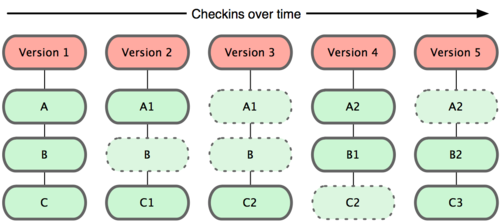
\includegraphics[width=10cm,keepaspectratio]{data/GitRevisionModel.png}

    每个版本都是对这个项目的快照(snapshot)。
\end{frame}

\begin{frame}
    \frametitle{其他系统的版本控制模型}
    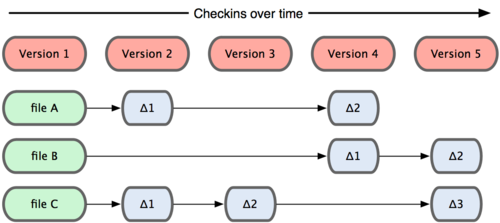
\includegraphics[width=10cm,keepaspectratio]{data/OtherRevisionModel.png}
\end{frame}

\begin{frame}
    \frametitle{分布式工作流程\footnote{\url{http://git-scm.com/book/en/Distributed-Git-Distributed-Workflows}}}
    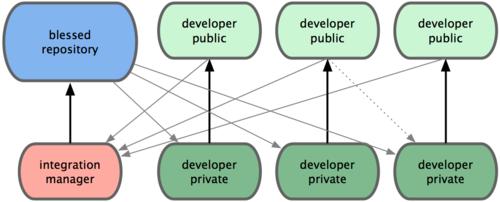
\includegraphics[width=10cm,keepaspectratio]{data/GitDistributedWorkflow.png}
    \begin{block}{我们的开发模式}
        \begin{itemize}
            \item 公共的仓库,由管理员负责
            \item 个人的仓库,由开发者自己管理
            \item 如果要将个人的代码合并如公共的仓库,
                  提交Pull Request,告诉管理员仓库的url和分支名。
        \end{itemize}
    \end{block}
\end{frame}

\begin{frame}
    \frametitle{Git的数据流}
    \begin{columns}
        \column{6.0cm}
            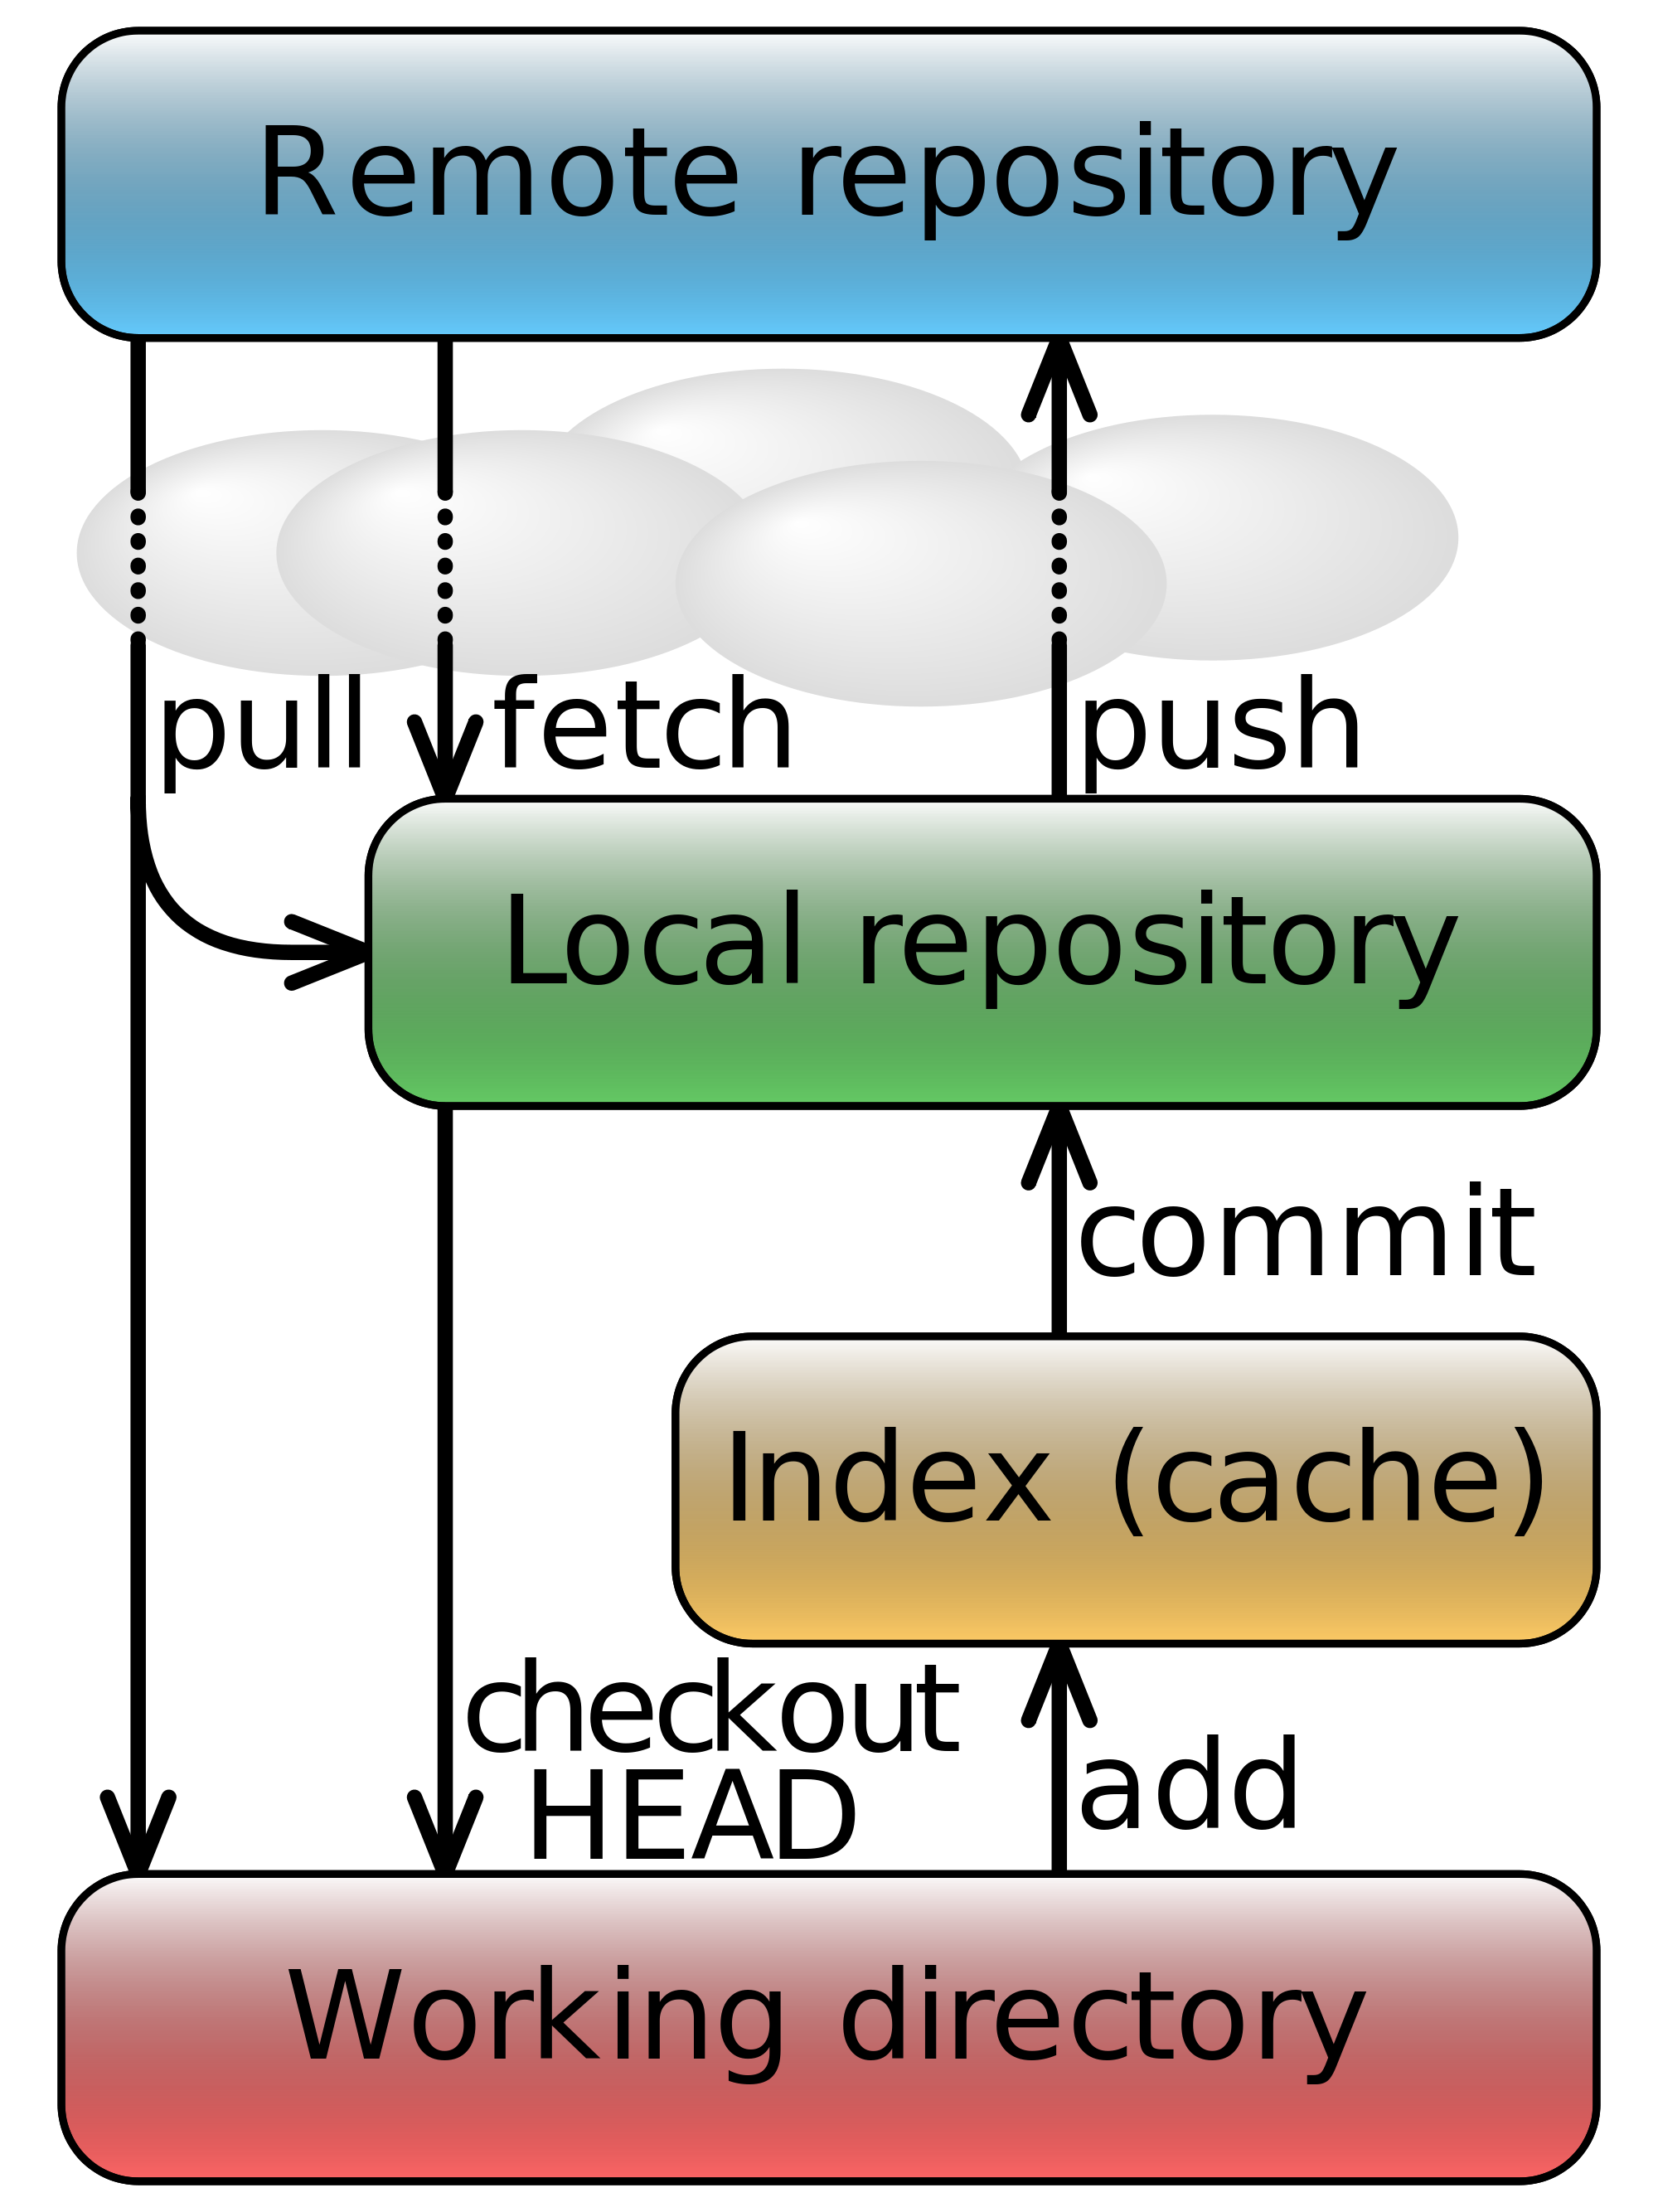
\includegraphics[height=8cm,keepaspectratio]{data/GitDataFlowSimplified.png}
            \label{pic:DataFlow}
        \column{4.5cm}
            \begin{itemize}
                \item 远程仓库
                \item 本地仓库
                \item 工作目录
            \end{itemize}
    \end{columns}
\end{frame}

\begin{frame}
    \frametitle{Git与CVS的部分区别
        \footnote{\scriptsize \url{http://stackoverflow.com/questions/802573/difference-between-git-and-cvs}}}
    \begin{block}{Git}
        \begin{itemize}
            \item 分布式仓库。用户无需任何服务器,在本地即可进行所有操作。
            \item 原子操作。操作要么完全成功,要么完全失败。
            \item 改动是对于整个项目。因此很容易回退到特定版本。
            \item 版本号也是基于整个项目。一个版本对应一个快照。
            \item 分支功能强大。包括创建合并等。
        \end{itemize}
    \end{block}
    \begin{block}{CVS}
        \begin{itemize}
            \item 集中式仓库。需要设置仓库的服务器,合并等操作都由服务器完成。
            \item 非原子操作。如果某个操作在中间被打断,可能处于不一致的状态。
            \item 改动是对于一个文件而言。我们可以checkout一些特定的文件。
            \item 版本号是对于文件而言。我们需要建立tag关联各个文件,
                  以指向特定的状态。
        \end{itemize}
    \end{block}
\end{frame}

\begin{frame}
    \frametitle{Git与SVN的部分区别
        \footnote{\scriptsize \url{http://stackoverflow.com/questions/871/why-is-git-better-than-subversion}}}
        \begin{quote}
            Git is not better than Subversion. But is also not worse. It's
            different.
        \end{quote}

        \begin{quote}
            The key difference is that it is decentralized.
        \end{quote}

        \begin{quote}
            Git has the advantage that it's MUCH better suited if some
            developers are not always connected to the master repository. Also,
            it's much faster than SVN. And from what I hear, branching and
            merging support is a lot better (which is to be expected, as these
            are the core reasons it was written).
        \end{quote}

        \begin{quote}
            SVN creates .svn directories in every single folder (Git only
            creates one .git directory). Every script you write, and every grep
            you do, will need to be written to ignore these .svn directories.
            You also need an entire command ("svn export") just to get a sane
            copy of your files.
        \end{quote}
\end{frame}

\begin{frame}
    \frametitle{Git使用时的建议\footnote{\scriptsize 仅为个人意见}}
    \begin{itemize}
        \item 为你的代码创建一个git仓库。可以只在本地。
              对可以公开的代码,可以托管于github等网站。
        \item 追踪你的代码。经常commit你的改动。
        \item 研究某一个新特性时,建立分支。最好基于主干创建分支。
        \item 多查资料。网上总有解答。
    \end{itemize}
    \begin{block}{我的一些经历体验}
        \begin{itemize}
            \item 在Dayabay SVN的people中提交过多commit,
                  导致邮件列表中出现太多的消息。导致不敢随时commit工作。
            \item 半年的Dyb2Sim开发,没有遇到太多git相关的问题。
                  唯一一次有难度的,是对geant4 9.4 和 9.5的同时支持。
                  因为geant4本身接口的变动,使得9.5环境下不可以直接编译9.4的代码。
                  开发某一个新特性时,是基于9.4,然后需要移到9.5。
                  git的一条merge命令就搞定了。
        \end{itemize}
    \end{block}
\end{frame}

\section{Trac}
    %!Mode:: "TeX:UTF-8"
%\begin{frame}
%    \frametitle{OUTLINE}
%    \begin{itemize}    
%        \item
%    \end{itemize}
%\end{frame}

\begin{frame}
    \begin{center}
        \LARGE \tt{TRAC}
    \end{center}
\end{frame}

\begin{frame}
    \frametitle{为何用trac?}
    \begin{itemize}    
        \item 目前的地址:
        \item \url{http://dyb2app1.ihep.ac.cn/trac}
        \item 需要汇总各种信息
            \begin{itemize}
                \item 包括一些Wiki信息
                \item BUG的汇报
                \item 今后的打算
            \end{itemize}
    \end{itemize}
\end{frame}

\begin{frame}
    \frametitle{Wiki}
    \begin{itemize}    
        \item 这里的功能大家自己摸索
        \item 一些有趣的功能
            \begin{itemize}
                \item 插入代码
                \item 可支持
                    \begin{itemize}
                        \item c
                        \item cpp
                        \item python
                        \item 甚至是diff
                    \end{itemize}
                \item Workflow
            \end{itemize}
    \end{itemize}
\end{frame}

\newsavebox{\TracWikiCode}
\begin{lrbox}{\TracWikiCode}
\begin{lstlisting}
{{{#!cpp

class A{
};

}}}
\end{lstlisting}
\end{lrbox}

\begin{frame}
    \frametitle{插入代码}
    \par\usebox{\TracWikiCode}
\end{frame}

\newsavebox{\TracWikiWorkflow}
\begin{lrbox}{\TracWikiWorkflow}
%\begin{adjustbox}{width=\textwidth,height=10cm,keepaspectratio}
\begin{lstlisting}
{{{#!Workflow

read_public_admin = dyb2app1 -> gitadmin
read_public_user = dyb2app1 -> user

read_users_admin = users -> gitadmin
read_users_user = users -> user

write_public_repo = gitadmin -> dyb2app1
write_users_repo = user -> users

}}}
\end{lstlisting}
%\end{adjustbox}
\end{lrbox}

\begin{frame}
    \frametitle{Wiki中Workflow的代码}
    \par\usebox{\TracWikiWorkflow}
\end{frame}

\begin{frame}
    \frametitle{Wiki中Workflow的效果}
    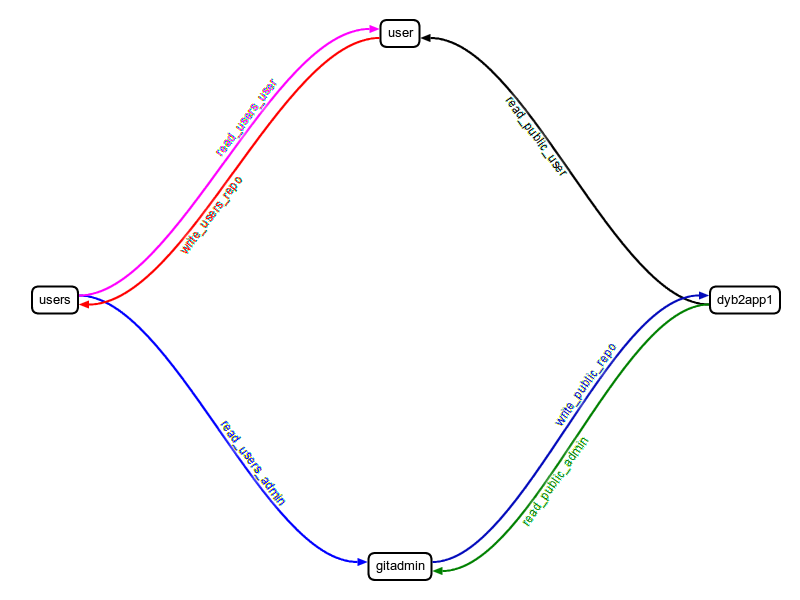
\includegraphics[width=10cm,keepaspectratio]{data/TracWorkflow.png}
\end{frame}

\begin{frame}
    \frametitle{Ticket的用处}
    \begin{itemize}    
        \item 向大家报告程序中的Bug
        \item 搜索有没有类似的Bug
        \item 设定下一步目标
        \item 例如,要进行一个新的探测器原型的开发
            \begin{itemize}
                \item 创建一个ticket,说明目标
                \item 得到的ticket的id
                \item 在个人仓库中建立一个相应ticket的分支
            \end{itemize}
    \end{itemize}
\end{frame}

\begin{frame}
    \frametitle{关于Ticket ID的妙用}
    \begin{itemize}    
        \item 例如,这个ticket的id为10。
        \item 在wiki中,可以用\tt{\#10}指向这个ticket。
        \item 在工作目录中,在\tt{commit}的内容中,也可以
              使用\tt{\#10}。
        \item \tt{\scriptsize{git commit -am "Finish Ticket \#10."}}
        \item Trac中,自动为\tt\textcolor{red}{{\sout{\#10}}} 创建了链接。
    \end{itemize}
\end{frame}

\begin{frame}
    \frametitle{创建Ticket}
    \begin{itemize}    
        \item 创建Ticket时,如果是汇报bug,请尽量贴出有用信息。
        \item 另外,好的习惯是,把这个Ticket中的信息补充完整。
        \item 例如,对于component来说,如果在开发DetSimX,
              那么就选择\tt{dyb2sim DetSimX}。
        \item 如果选项中的条目不完善,请告知管理员
    \end{itemize}
\end{frame}

\begin{frame}
    \frametitle{Milestone(在Roadmap中)}
    \begin{itemize}    
        \item 概念?
        \item Trac中的Milestone,不是以一个时间段作为标记。
        \item 而是以完成的Ticket做为标记。
        \item 因此,ticket中信息填全有助于我们了解项目的进展。
    \end{itemize}
\end{frame}

\begin{frame}
    \frametitle{Trac小结}
    \begin{itemize}    
        \item 遇到问题时,先搜索有没有类似的问题
        \item 如果能找到,看看是否已经修改了这个bug
        \item 如果没有,请尽快告知大家
        \item 以issue的形式,记录新的工作
        \item 与大家分享你的工作进展
    \end{itemize}
\end{frame}


\section*{end}
\begin{frame}
    \begin{center}
        \LARGE Q \& A
    \end{center}
\end{frame}

\end{document}
